\documentclass[11pt]{beamer}
\usetheme{Warsaw}
\usepackage[utf8]{inputenc}
\usepackage[spanish]{babel}
\usepackage{amsmath}
\usepackage{amsfonts}
\usepackage{amssymb}
\usepackage{graphicx}
\usepackage{ragged2e}
\usepackage{caption}
\setbeamertemplate{caption}[numbered]
\spanishdecimal{.}

\justifying
\author[Oscar - David \hspace{22.5mm}]{Oscar Joel Castro Contreras \\ David Peralez Olguin}
\title[\hspace{26mm} \insertframenumber]{Probabilidad y Estadística}
%\setbeamercovered{transparent} 
%\setbeamertemplate{navigation symbols}{} 
%\logo{} 
\institute{Universidad Autónoma de Coahuila} 
\date{7 de junio de 2022} 
%\subject{} 
\begin{document}

     \usebackgroundtemplate{
          
\includegraphics{Fondo .png}}

	\begin{frame}
		\titlepage
	\end{frame}

	\begin{frame}
		\tableofcontents
	\end{frame}

%──────────────────────────────────────────────────────────────────────────────────────────────────────────────────────────────────────────

	\section{Introducción}
		\begin{frame}{Introducción}
			Las aplicaciones de la probabilidad para describir el comportamiento de los fenómenos son 
			variados, para este caso se hizo uso de la distribución normal aplicada a una situación cotidiana o 
			recreativa como lo es el hacer palomitas de maíz en un horno de microondas, lo esencial es saber 
			que debido a diversos factores, no se obtendrán el $ 100\% $ de las palomitas, habrá semillas sin 
			reventar. Fue en base a esto que se realizó este proyecto.
		\end{frame}
		
%──────────────────────────────────────────────────────────────────────────────────────────────────────────────────────────────────────────

	\section{Objetivos}
		\begin{frame}{Objetivos}
			\begin{block}{}
				\begin{enumerate}
					\vspace{0.5cm}
					\item Analizar experimentalmente la relación de las palomitas sin hacer en relación con el total de una 
						 bolsa.
					\vspace{0.5cm}
					\item Calcular su probabilidad por medio de la aproximación de la binomial a la normal.
					\vspace{0.5cm}
				\end{enumerate}
			\end{block}
		\end{frame}

%──────────────────────────────────────────────────────────────────────────────────────────────────────────────────────────────────────────

	\section{Datos}
		\begin{frame}{Datos}
			\begin{table}[h!]
				\centering
				\begin{tabular}{|c|c|c|c|}
					\hline
					Bolsa De & Palomitas & Palomitas & Porcion De \\
					Palomitas & Hechas & No Hechas & Bolsa No Hecha \\\hline
					$ 1 $ & $ 295 $ & $ 75 $ & $ 0.2027 $ \\\hline
					$ 2 $ & $ 260 $ & $ 110 $ & $ 0.2972 $ \\\hline
					$ 3 $ & $ 279 $ & $ 91 $ & $ 0.2459 $ \\\hline
					$ 4 $ & $ 249 $ & $ 121 $ & $ 0.3270 $ \\\hline
					$ 5 $ & $ 250 $ & $ 120 $ & $ 0.3243 $ \\\hline
					$ 6 $ & $ 310 $ & $ 60 $ & $ 0.1621 $ \\\hline
					$ 7 $ & $ 302 $ & $ 68 $ & $ 0.1837 $ \\\hline				
				\end{tabular}
			\end{table}
		\end{frame}

		\begin{frame}{Datos}
			\begin{block}{Porción Por Palomitas}
				$$ \mu = \frac{\displaystyle\sum_{i=1}^{n} x_i}{n} = 92.14 $$
				$$ \sigma = \sqrt{\frac{\displaystyle\sum_{i=1}^{n} (x_i-\mu)^2}{n}} = 25.29 $$
			\end{block}
		\end{frame}

		\begin{frame}{Datos}
			\begin{block}{Porción Por Bolsa}
				$$ \mu = \frac{\displaystyle\sum_{i=1}^{n} x_i}{n} = 0.24 $$
				$$ \sigma = \sqrt{\frac{\displaystyle\sum_{i=1}^{n} (x_i-\mu)^2}{n}} = 0.068 $$
			\end{block}
		\end{frame}

%──────────────────────────────────────────────────────────────────────────────────────────────────────────────────────────────────────────

	\section{Problemas}
		\begin{frame}{Problema 1}
			\begin{block}{$ \left( 1 \right) $ ¿Cuál es la probabilidad de que $ 1/3 $ o menos de la bolsa sea de palomitas no hechas?}
				$$ \mu = 0.24 \quad \sigma = 0.068 $$
				$$ \overline{x} \leq \frac{1}{3} $$
				$$ z = \frac{\overline{x} - \mu}{\sigma} = \frac{1/3 - 0.24}{0.068} = 1.37 $$
				$$ P(z \leq 1.37) = 0.9147 $$
			\end{block}
		\end{frame}

		\begin{frame}
			\begin{figure}[H]
				\centering
				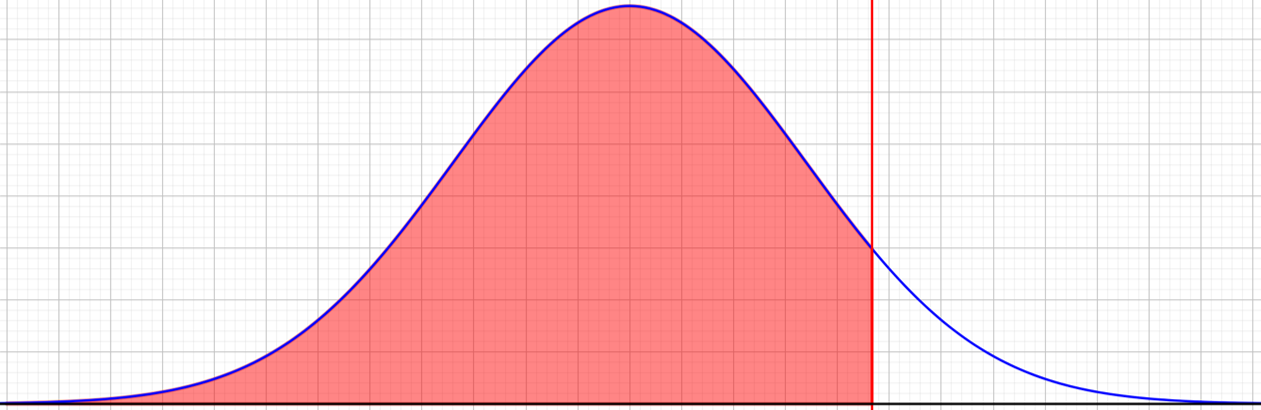
\includegraphics[width=\linewidth]{Imagen1.png}
				\caption{Área bajo la curva en $ z \leq 1.37 $}
			\end{figure}
		\end{frame}

		\begin{frame}{Problema 2}
			\begin{block}{$ \left( 2 \right) $ ¿Cuál es la probabilidad de que más de 1/5 de la bolsa sea de palomitas no hechas?}
				$$ \mu = 0.24 \quad \sigma = 0.068 $$
				$$ \overline{x} > \frac{1}{5} $$
				$$ z = \frac{\overline{x} - \mu}{\sigma} = \frac{1/5 - 0.24}{0.068} = -0.59 $$
				$$ P(z > -0.59) = 1 - P(z \leq -0.59) = 1 - 0.2776 = 0.7224 $$
			\end{block}
		\end{frame}

		\begin{frame}
			\begin{figure}[H]
				\centering
				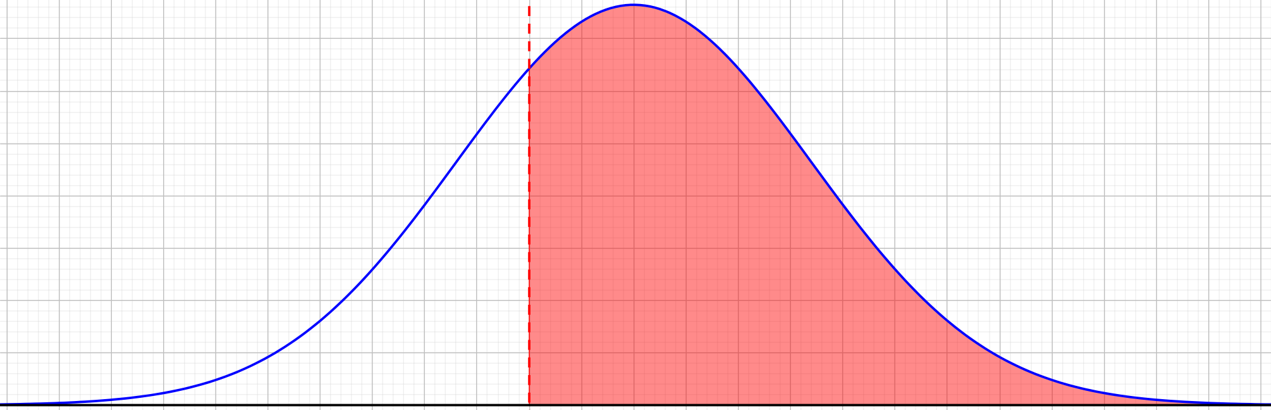
\includegraphics[width=\linewidth]{Imagen2.png}
				\caption{Área bajo la curva en $ z > -0.59 $}
			\end{figure}
		\end{frame}

		\begin{frame}{Problema 3}
			\begin{block}{$ \left( 3 \right) $ ¿Cuál es la probabilidad de que más de 1/4 pero menos de 2/5 de la bolsa sea de palomitas no hechas?}
				$$ \mu = 0.24 \quad \sigma = 0.068 $$
				$$ \overline{x_1} > \frac{1}{4} \quad \overline{x_2} < \frac{2}{5}  $$
				$$ z_1 = \frac{\overline{x} - \mu}{\sigma} = \frac{1/4 - 0.24}{0.068} = 0.15 $$
				$$ z_2 = \frac{\overline{x} - \mu}{\sigma} = \frac{2/5 - 0.24}{0.068} = 2.35 $$
				$$ P(0.15 < z < 2.35) = P(z \leq 2.35) - P(z \leq 0.15) = $$
				$$ 0.9906 - 0.5596 = 0.4310 $$
			\end{block}
		\end{frame}

		\begin{frame}
			\begin{figure}[H]
				\centering
				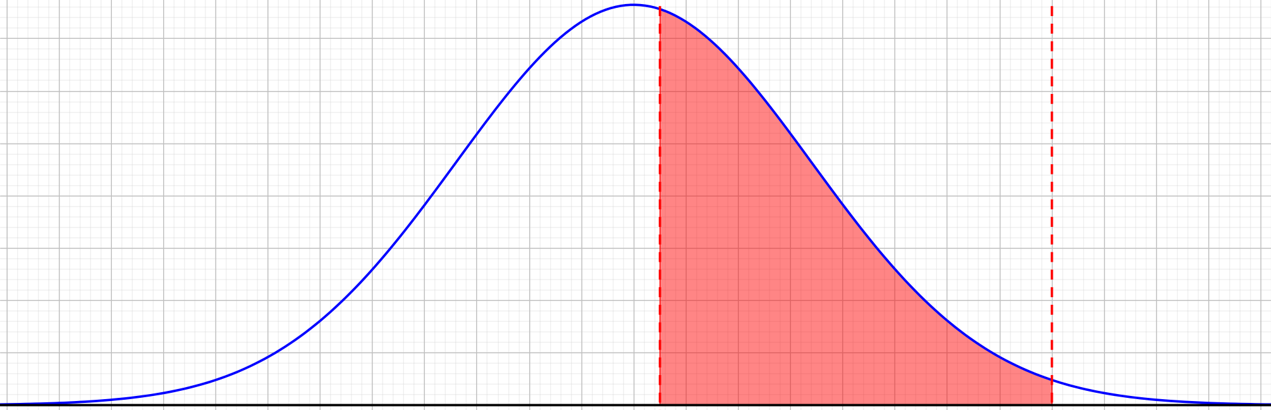
\includegraphics[width=\linewidth]{Imagen3.png}
				\caption{Área bajo la curva en $0.15 < z < 2.35 $}
			\end{figure}
		\end{frame}

%──────────────────────────────────────────────────────────────────────────────────────────────────────────────────────────────────────────
	
	\section{Conclusión}
			\begin{frame}{Conclusión}
				\begin{itemize}
					\item La probabilidad de que $ 1/3 $ de la bolsa no se haga o de que queden $ 123 $ palomitas no hechas es de $ 91.47\% $
     				\item La probabilidad de que más $ 1/5 $ de la bolsa no se haga o de que queden más de $ 74 $ palomitas no hechas es de $ 72.24\% $
         				\item La probabilidad de que más de $ 1/4 $ pero menos de $ 2/5 $ de la bolsa no se haga o que queden mas de $ 92 $ pero menos de $ 148 $ palomitas no hechas es de $ 43.10\% $
				\end{itemize}
			\end{frame}

%──────────────────────────────────────────────────────────────────────────────────────────────────────────────────────────────────────────

	\section{Referencias}
		\begin{frame}{Referencias}
			\centering
			\begin{thebibliography}{10}
				\bibitem{bib:item1} Walpole, R. E. (2012). PROBABILIDAD Y ESTADISTICA PARA INGENIERIA Y CIENCIAS (9.a ed.). PEARSON EDUCACION.
			\end{thebibliography}
		\end{frame}

\end{document}